\begin{multicols}{3}[\section{IEEE 802.11 Basics}]

\rhead{Autor: Jan Selig}
\lfoot{Letzte Bearbeitung: 11.04.2016}

\newrefsegment

\begin{boxedminipage}{\linewidth}
\begin{tabular}{p{2,1 cm}p{2.7 cm}}
\textbf{Steckbrief}& \\
\end{tabular}
\begin{tabular}{p{2,1 cm}|p{2.7 cm}}
      Einsatz seit & 1997\\
      \hline
      Frequenz"-bereich  & \SI{2.4}{\giga\hertz}, \SI{5}{\giga\hertz} \\
      \hline
      Datenrate & \SI{2}{Mbit/s} - \SI{54}{Mbit/s}\\
      \hline
       Verbreitung & Weltweit\\
      \hline
      Reichweite & ca. \SI{20}{\metre}\\
\end{tabular}
\end{boxedminipage}
\par
%Source http://www.fh-bingen.de/fileadmin/user_upload/Lehrende/Kilsch_Dieter/internet/projekte/TedoSchStiUnits.pdf -> Seite 9 findet ihr alle verwendbaren Einheiten, wie:
%\SI{Zahl}{\mega\hertz} oder \SI{Zahl}{\mili\metre}
%Ich weiß ehrlich gesagt nicht welche Einheiten ihr im Text genau braucht, aber in dem Dokument und mit obigen Beispiel sollte es umsetzbar ein.
\subsection*{Überblick}

IEEE 802.11 definiert die Bitübertragungsschicht und die Sicherungsschicht des ISO/OSI-Schichtenmodells für ein drahtloses Netzwerk.
Insgesamt setzt sich der IEEE 802.11 Standard aus 12 Erweiterungen zusammen, die sich größtenteils in der  Übertragungsgeschwindigkeit,  Modulation des Trägersignals und Anpassungen an verschiedene Länder unterscheiden. Zu den Basics zählen allerdings nur 802.11, 802.11a, 802.11b, 802.11h, 802.11j und 802.11g. 
Der reine 802.11 Standard ist veraltet und wird in der Praxis nicht mehr verwendet.


\subsection*{Technische Erläuterungen}
\subsubsection*{Architekturen}  
Es sind im Standard 802.11 grundsätzlich drei verschiedene Architekturen vorgesehen, wie ein drahtloses Netzwerk aufgebaut werden kann. Diese sind in Abbildung  \ref{fig:IEEE802.Architektur} dargestellt. Der Regelfall ist die Anbindung von Kommunikationsgeräten über einen sogenannten Access Point oder auch Basisstation genannt. Dieser AP stellt eine Schnittstelle zwischen kabellosen Kommunikationsgeräten und einem bestehenden lokalen Netzwerk dar. Die zweite Architektur beschreibt den Aufbau eines Netzwerkes mit mehreren Kommunikationsgeräten ohne den Einsatz von AP’s. Hierbei wird ein sogenanntes Ad-Hock-Netzwerk aufgebaut, bei dem alle Kommunikationsgeräte untereinander drahtlos verbunden sind. Die letzte Architektur sieht eine Richtfunkstrecke über eine maximale Distanz von 10 Kilometern vor. ~\cite{basics.3}
\begin{Figure}
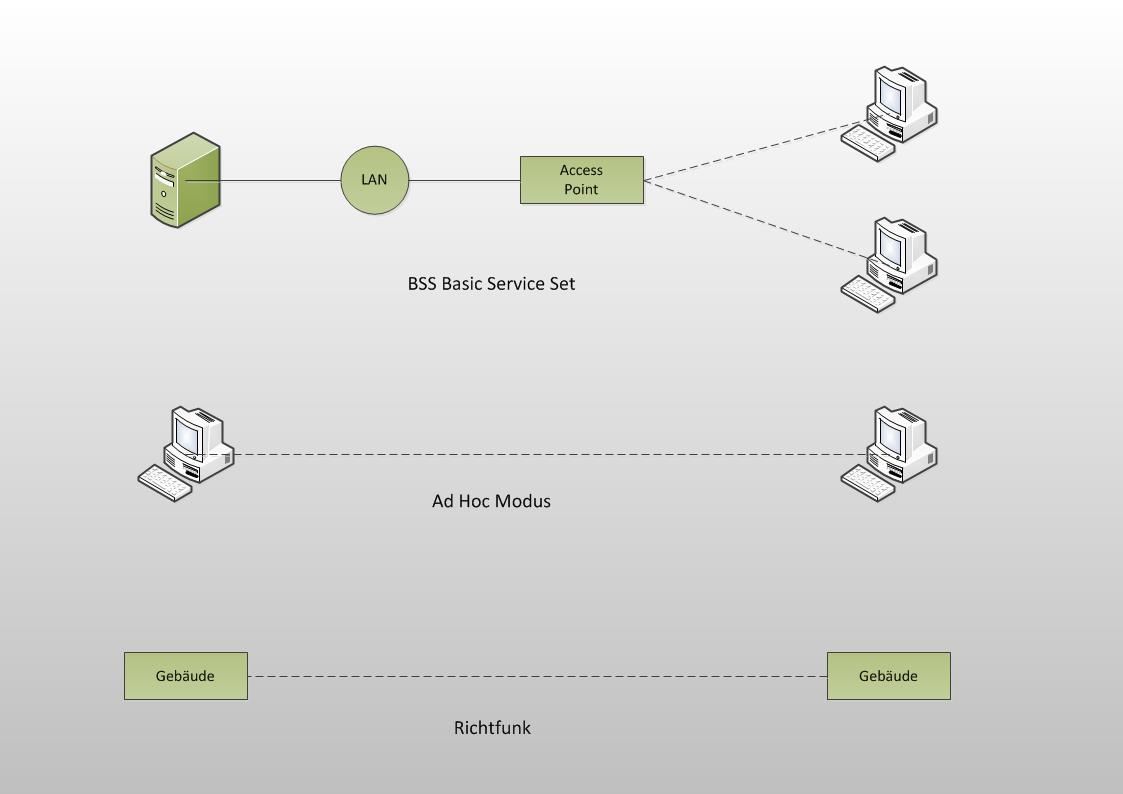
\includegraphics[width=\linewidth]{Kapitel/IEEE802.11/Grafiken/80211_Architektur.jpg}
\captionof{figure}{IEEE 802.11 Architektur~\cite{basics.5}}
\label{fig:IEEE802.Architektur}
\end{Figure}

\subsubsection*{Frequenzen und Kanäle}  
Für ein drahtloses Netzwerk stehen drei Frequenzbereiche zur Verfügung: 2,4 GHz, 5 GHz und 60 GHz. Der Standard 802.11 nutzt den Frequenzbereich 2,4 GHz, das sogenannte ISM-Band. Dieser Frequenzbereich ist lizenzfrei, also frei nutzbar. Die Tatsache, dass das ISM Band lizenzfrei ist, bedeutet aber auch, dass sich in diesem Frequenzbereich auch andere Funknetze aufhalten können. Die Geschwindigkeit und Stabilität eines Funknetzwerks mit IEEE 802.11 hängt folglich von der Intensität der Nutzung anderer Funktechniken im gleichen Frequenzband ab. 

Da sich in einem drahtlosen Netzwerk alle Teilnehmer das Übertragungsmedium teilen müssen und dieses nicht vollständig belegt sein darf, teilt man das Frequenzband zusätzlich in sogenannte Kanäle ein, die mit anderen Netzen geteilt werden müssen. Im 2,4-GHz-Frequenzband existieren insgesamt 79 schmalbandige Kanäle, die in mehrere breitbandige Kanäle zusammengefasst sind. Die Anzahl an Kanälen kann sich aber von Land zu Land unterscheiden. In Europa gibt es 13 solcher Kanäle. Da diese allerdings eng aneinandergereiht und überlappend sind, kann man nicht alle der Kanäle verwenden, sondern je nach Kanalverteilung nur 3 oder 4. ~\cite{basics.4}

In den Abbildugen \ref{fig:IEEE802.Frequenzbereich} und \ref{fig:IEEE802.Frequenzkanäle} werden nochmals die Basisinformationen zu den Frequenzbereichen und zu den Frequenzkanälen dargestellt.

\begin{Figure}
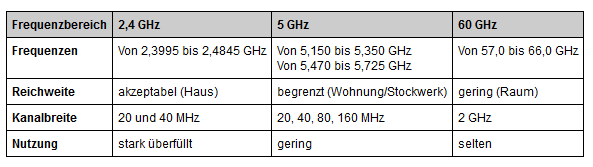
\includegraphics[width=\linewidth]{Kapitel/IEEE802.11/Grafiken/Frequenzbereiche_80211X.png}
\captionof{figure}{IEEE 802.11 Frequenzbereiche~\cite{basics.7}}
\label{fig:IEEE802.Frequenzbereich}
\end{Figure}

\begin{Figure}
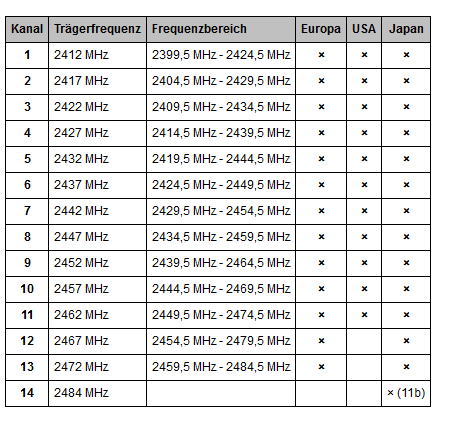
\includegraphics[width=\linewidth]{Kapitel/IEEE802.11/Grafiken/Traegerfrequenz.png}
\captionof{figure}{IEEE 802.11 Trägerfrequenz~\cite{basics.7}}
\label{fig:IEEE802.Frequenzkanäle}
\end{Figure}

\subsubsection*{Übertragungstechnik}
Da ein drahtloses Netzwerk grundsätzlich ein Broadcast Medium ist, kann es bei gleichzeitigen Übertragungen zu sogenannten Kollisionen kommen. Mit Kollisionen ist eine Überlagerung der Funksignale gemeint. Um diese Kollisionen zu vermindern, gibt es ein bestimmtes Zugriffsverfahren, das als Carrier Sense Multiple Access bezeichnet wird. CSMA sieht vor, dass jeder Kommunikationsteilnehmer vor dem Senden prüfen muss, ob das Übertragungsmedium frei ist. 

Zur Übertragung von Signalen wird die Spread-Spectrum-Technologie verwendet. Spread Spectrum Systeme können Distanzen von ca. 250 Metern überbrücken. Je größer die Entfernung zwischen Kommunikationsgerät und AP, desto kleiner der Durchsatz. Die Funktionsweise ist hierbei wie folgt: Die zu übertragende Information wird vom Sender über mehrere Kanäle verteilt. Die Wahl der Kanäle folgt einem zufälligen Muster. Es gibt zwei Varianten zur Nutzung des Spread Spectrums, die im Standard 802.11 definiert sind:

Bei der sogenannten \textit{Frequency Hopping Spread Spectrum} Technologie (Abbildung  \ref{fig:IEEE802.Frequenzhopping}) nutzen
Sender und Empfänger für die Übertragung 79 Kanäle. Durch die Vergabe einer bestimmten Hopping-Sequence werden die Kanäle nach einem Zufallsmuster gewechselt. Somit wird die eigentliche Information über mehrere Frequenzen verteilt zum Empfänger gesendet. 
\begin{Figure}
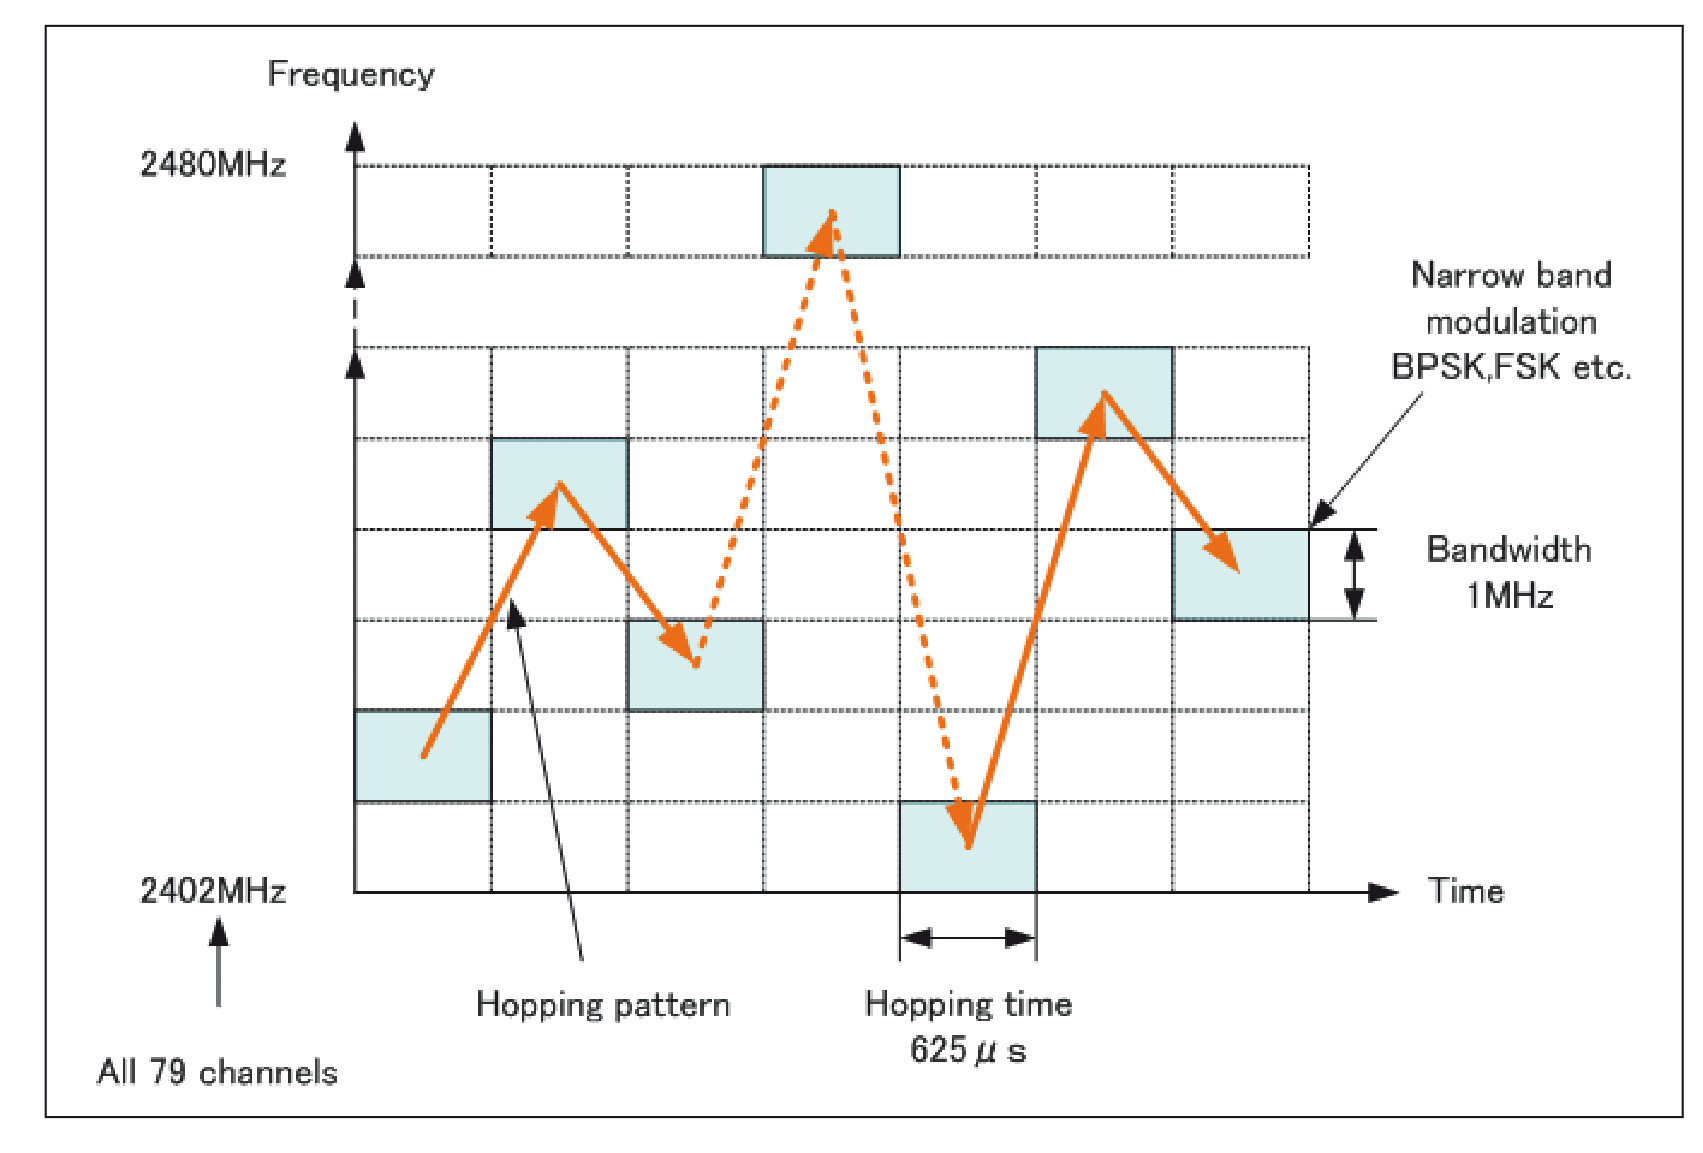
\includegraphics[width=\linewidth]{Kapitel/IEEE802.11/Grafiken/Frequenzhopping.png}
\captionof{figure}{Spread Sprectrum Frequenzhopping~\cite{basics.6}}
\label{fig:IEEE802.Frequenzhopping}
\end{Figure}

Die zweite Technologie, genannt \textit{Direct Sequence Spread Spectrum},
arbeitet mit einer festen, aber wählbaren Frequenz. Es stehen insgesamt 14 Kanalgruppen mit einer Bandbreite von je 22 MHz zur Verfügung. 
~\cite{basics.4}


\subsection*{Einsatz}
Für drahtlose Netzwerke gibt es zahlreiche Anwendungszwecke, von denen an dieser Stelle nur einige genannt werden:
\begin{itemize}
	\item Drahtlose Netzwerke ermöglichen eine hohe Mobilität
	\item Drahtlose Netzwerke bieten  eine Ergänzung zum 				kabelgebundenen Ethernet und ermöglichen zum Beispiel in Firmen  die mobile Nutzung der Arbeitsrechner
	\item Mobile Geräte können einfach, ohne Verkabelung und unabhängig vom Ort via Funk miteinander vernetzt werden
	\item Drahtlose Netzwerke können bei schwierigen Verkabelungsverhältnissen eingesetzt werden wie z.B. Denkmalschutz eines Gebäudes~\cite{basics.8}
\end{itemize}

\subsection*{Sicherheit}

Da kabellose Übertragungen Broadcast-Verbindungen sind, bieten diese einfach ausnutzbare Sicherheitslücken. Um dies zu verhindern enthält der 802.11 Standard ein Verschlüsselungsschema namens Wired Equivalent Privacy. WEP stellt hierfür Funktionen für die Authentifizierung und Verschlüsselung bereit.
Jedoch bietet dieses Schema zu viele Schwachstellen und gilt seit 2001 als unsicher. Aus diesem Grund wurde es durch andere Schemata wie z.B. WiFi Protected Access und WiFi Protected Access 2 ersetzt.~\cite{basics.2}

\end{multicols}
\newpage
\section*{Historische Entwicklung}
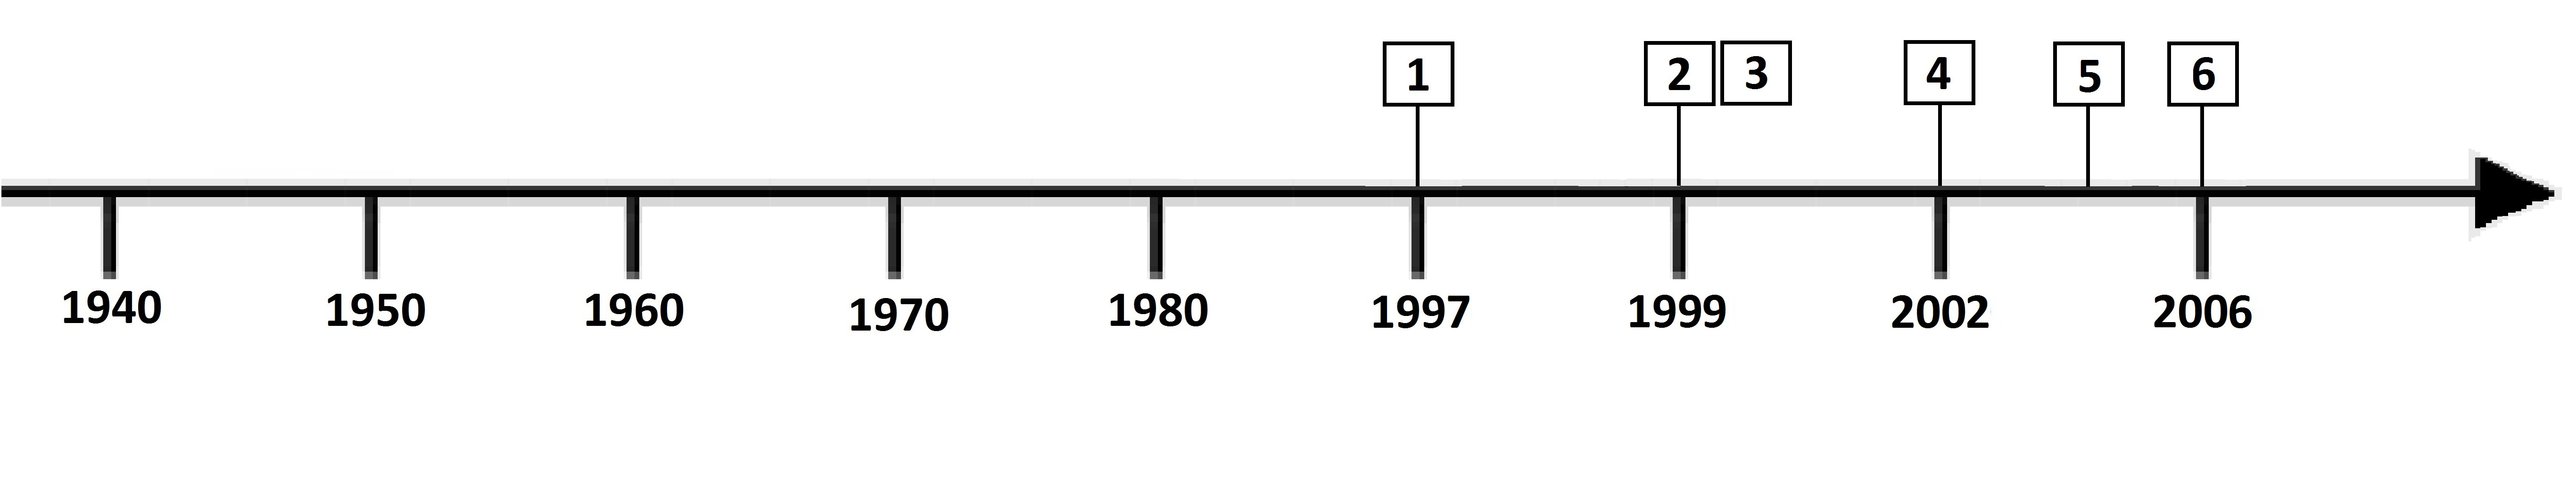
\includegraphics[width=\textwidth]{Kapitel/IEEE802.11/Grafiken/Zeitstrahl_2}
\par
\noindent
\begin{tabular}{|p{1 cm}|p{3 cm}|p{13.55 cm}|}
	\hline
	Nummer & Datum & Entwicklungsschritte~\cite{basics.1}\\
	\hline
	1 & 1997 &  Erstmalige Spezifizierung einer verbindlichen Luftschnittstelle für lokale Funknetzwerke. Dieser Standard wird als IEEE 802.11 bezeichnet und erlaubt Datenraten von bis zu 2 MBits/s brutto.\\
	\hline
	2 & 1999 & Erweiterung zum Standard IEEE 802.11b, der höhere Datenraten von bis zu 11 MBit/s brutto bietet und das gleiche Modulationsverfahren benutzt, wie sein Vorgänger.\\
	\hline
	3 & 1999 & Verabschiedung des Standards IEEE 802.11a. Dieser ermöglicht größere Datenraten von bis zu 54 MBits/s brutto, nutzt das 5Ghz Frequenzband und das orthogonale Frequenzmultiplexverfahren zur Modulation des Übertragungssignals. Dieses Verfahren war zu dieser Zeit jedoch  nur für das 5GHz Frequenzband freigegeben.\\
	\hline
	4 & 2002 & Erst 2002 mit der Einführung des Standards 802.11g war dieses Modulationsverfahren auch für das 2,4 GHz Frequenzband verfügbar. 802.11g bietet Datenraten von bis zu 54 MBit/s brutto. Des Weiteren bietet dieser Standard auch noch eine Möglichkeit zur Kompatibilität mit Geräten, die noch den 802.11b Standard nutzen.\\
	\hline
	5 & 2004 & Der Standard 802.11j basiert auf dem Standard 802.11a und stellt eine Erweiterung für den japanischen Markt dar.\\
	\hline
	6 & 2006 & Der Standard 802.11h basiert ebenfalls auf dem Standard 802.11a und ist für den Betrieb mit großen Sendeleistungen gedacht.\\
	\hline
\end{tabular}
\par
\begin{multicols}{3}

%Dieser Kommentar ist vorerst zum Ignorieren gedacht. Er ist quasi gar nicht da. Hier wird kein Spaltenbreites Bild eingefügt. Nein. Wird es nicht.
%\end{multicols}
%\begin{FigureFullWidth}
%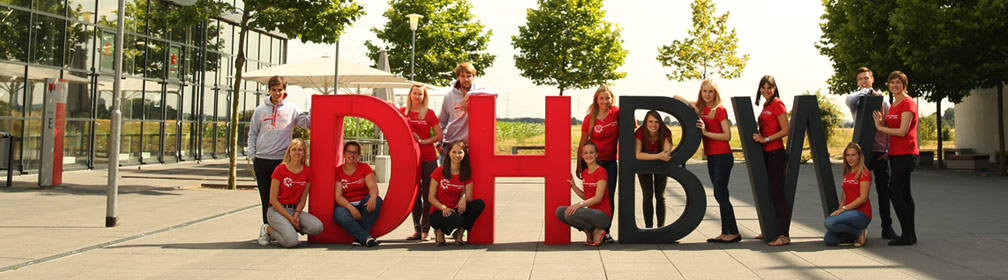
\includegraphics[width=\textwidth, height = 0.125\textheight]{Kapitel/Vorlage/Grafiken/966a49a.jpg}
%\captionof{figure}{DHBW-Startseitenbild~\cite{vorlage.9}}
%\end{FigureFullWidth}
%\begin{multicols}{3}

\subsection*{Anbieter und Gremien}
IEEE 802.11 bezeichnet einen von „Institute of Electrical and Electronics Engineers“ definierten Standard für drahtlose Netzwerke auf Basis von Ethernet. IEEE ist ein internationaler Berufsverband von Informationstechnikern, die unter anderem technische Standards spezifizieren. Einer der bekanntesten Standards ist der Standard 802.3, der die Netzwerkschnittstelle Ethernet spezifiziert.

\subsection*{Ausblick}
Mit dem Standard IEEE 802.11ac wurden bereits 2014 drahtlose Hochgeschwindigkeitsnetze spezifiziert, die eine Datenübertragungsrate von 600 Mbit/s ermöglichen. Weiterführend wäre zum Beispiel eine Technik, die Daten nicht per Funk, sondern per Licht optisch überträgt, wie die in Entwicklung befindliche Technik LiFi.
Ein weiterer Schritt in die Zukunft wird meiner Meinung nach jedoch nicht nur die Entwicklung von Technologien zur höheren Datenübertragung in drahtlosen Netzwerken sein, sondern eine vollständige Abstraktion von kabelgebundenen Medien. Dazu zählt die Verbindung von AP's zu Routern, kabelgebundene Verbindungen von Netzwerkkomponenten zu anderen Komponenten, aber auch beispielsweise HDMI- oder USB-Kabel.

\printbibliography[segment=1,heading=subbibliography]

\end{multicols}
\newpage